\chapter{Arrivals prediction: Hospital emergency room}


\section{Data}

The dataset contains accesses to the emergency room of the Maggiore Hospital in Bologna.

Each row of the dataset represents a patient and the features are:
\begin{descriptionlist}
    \item[\texttt{Triage}] Time of arrival.
    \item[\texttt{TKCharge}] Time of first visit.
    \item[\texttt{Code}] Priority (\texttt{white}, \texttt{green}, \texttt{yellow}, and \texttt{red}).
    \item[\texttt{Outcome}] Indicates whether the patient got admitted or left.
\end{descriptionlist}

\begin{description}
    \item[Binning] 
        As the problem is to predict the total number of arrivals at fixed intervals, binning can be used to obtain a dataset with an hour granularity.
\end{description}


\section{Approaches}

\begin{remark}
    MSE assumes that the conditional distribution of the predictions follows a normal distribution.
\end{remark}

\begin{remark}
    Arrivals usually follow a Poisson distribution as:
    \begin{itemize}
        \item There is a skew in the tail.
        \item All values are positive.
        \item Events are independent.
    \end{itemize}

    \begin{figure}[H]
        \centering
        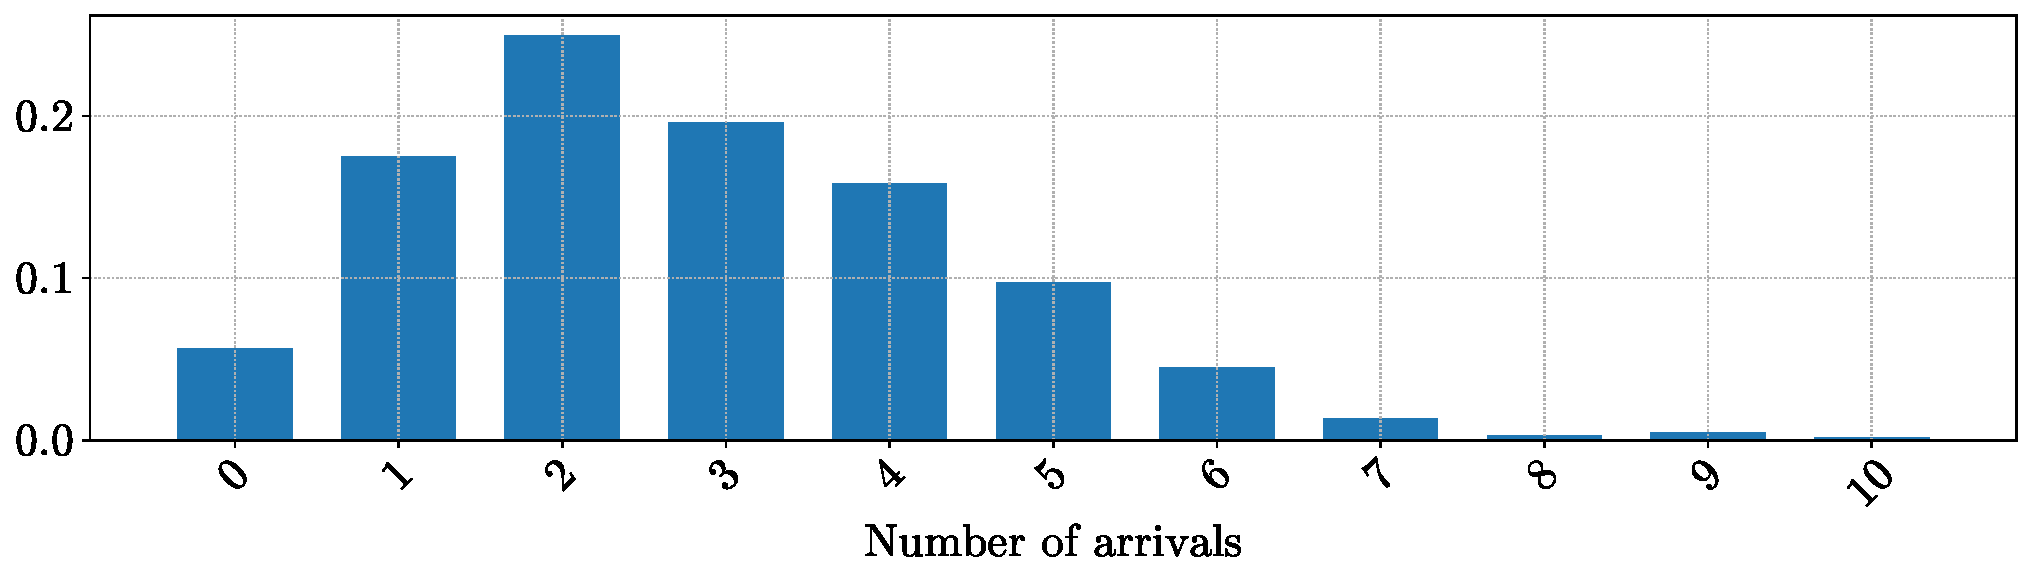
\includegraphics[width=0.8\linewidth]{./img/_skinwrapper_poisson.pdf}
        \caption{Arrivals distribution at 6 a.m.}
    \end{figure}

    \begin{theorem}
        If the inter-arrival time is exponential with respect to a fixed rate, the counts of the arrivals will always follow a Poisson distribution.
    \end{theorem}

    \begin{figure}[H]
        \centering
        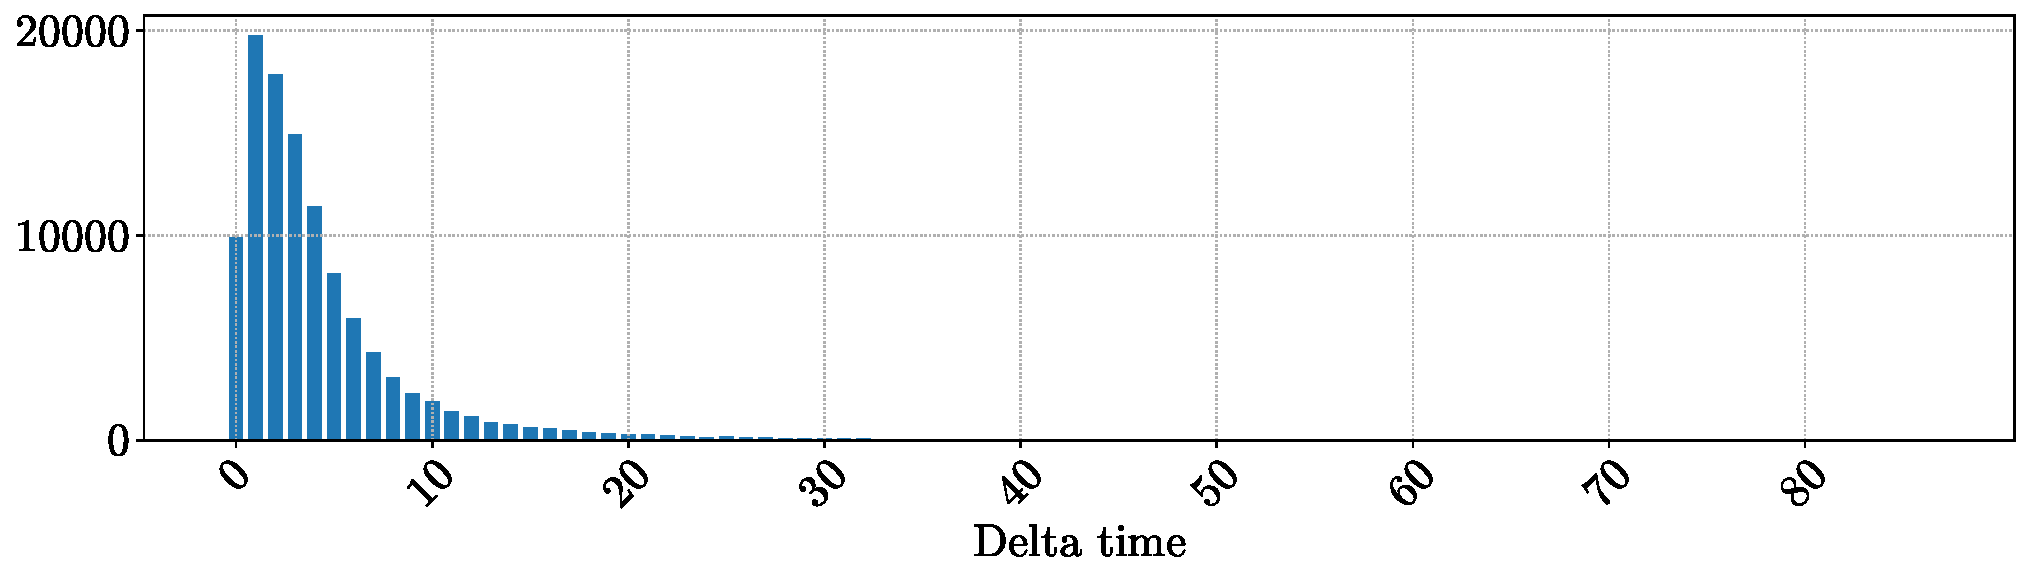
\includegraphics[width=0.8\linewidth]{./img/_skinwrapper_interarrival.pdf}
        \caption{Dataset inter-arrival counts (the first bar is due to binning artifacts)}
    \end{figure}
\end{remark}

\subsection{Neuro-probabilistic model}

\begin{description}
    \item[Poisson distribution] \marginnote{Poisson distribution}
        Distribution with discrete support whose probability mass function is defined as:
        \[ p(k, \lambda) = \frac{\lambda^k e^{-\lambda}}{k!} \]
        where $\lambda$ is the occurrence rate of the events.

        \begin{remark}
            Both mean and standard deviation of a Poisson distribution are $\lambda$.
        \end{remark}

        \begin{remark}
            $\lambda^{-\frac{1}{2}}$ represent the distribution skewness. For smaller values of $\lambda$, there is a positive skew to the left. For larger values of $\lambda$, the skew becomes less observable.
        \end{remark}

        \begin{remark}
            For this problem, $\lambda$ is the average number of arrivals in each bin.
        \end{remark}

    \item[Neuro-probabilistic model] \marginnote{Neuro-probabilistic model}
        Model that combines statistics and machine learning.

        \begin{remark}
            This class of models is known in the statistics literature as generalized linear model. With neural networks (i.e., non-linearity), they do not have an official name. ``Neuro-probabilistic model'' is an unofficial name.
        \end{remark}

        This problem can be formulated through the following probabilistic model:
        \[ y \sim \texttt{Poisson}(\lambda(x)) \]
        where $y$ is the number of arrivals and $\lambda(x)$ is the rate parametrized on the temporal information $x$.

        The rate can be approximated using an estimator as:
        \[ y \sim \texttt{Poisson}(\lambda(x, \theta)) \]
        where $\lambda(x, \theta)$ is a regression model.

        \begin{description}
            \item[Loss]
                Training is done for maximum likelihood estimation using the Poisson distribution:
                \[
                    \begin{split}
                        &\arg\min_\theta - \sum_{i=1}^{m} \log\left( f(y_i, \lambda(x_i, \theta)) \right) \\
                        &= \arg\min_\theta - \sum_{i=1}^{m} \log\left( \frac{\lambda(x_i, \theta)^{y_i} e^{\lambda(x_i, \theta)}}{y_i!} \right)
                    \end{split}
                \]

            \item[Architecture]
                Use an MLP to predict $\hat{\lambda}$ and then, instead of outputting the prediction directly, output a Poisson distribution object with rate $\hat{\lambda}$:
                \[
                    \begin{split}
                        \hat{\lambda} &= \texttt{MLP}(x) \\
                        \texttt{out} &= \texttt{Poisson}(\cdot, \hat{\lambda})
                    \end{split}
                \]

                Some considerations must be made:
                \begin{descriptionlist}
                    \item[Only positive rates] 
                        As $\hat{\lambda}$ must be positive, it is possible to combine a logarithm and an exponentiation to achieve this:
                        \[
                            \begin{split}
                                \log(\hat{\lambda}) &= \texttt{MLP}(x) \\
                                \texttt{out} &= \texttt{Poisson}\left( \cdot, \exp\left(\log(\hat{\lambda})\right) \right) = \texttt{Poisson}(\cdot, \hat{\lambda})
                            \end{split}
                        \]

                    \item[Standardization]
                        The input of the network can be standardized. On the other hand, standardizing the output is wrong as the Poisson distribution is discrete.

                        However, if the input is standardized (for training stability), the output of the network with normal weights initialization will have $0$ mean. Therefore, at the beginning, the network will predict $\hat{\lambda} \approx 1$ (i.e., the MLP predicts $\log(\hat{\lambda}) \approx 0$ and then $\hat{\lambda} = \exp\left(\log(\hat{\lambda})\right) \approx 1$) which might not be a reasonable starting point.

                        It is possible to provide an initial guess $\bar{\lambda}$ for $\hat{\lambda}$. This value can be used as a multiplicative factor, so that the first prediction will be close to $\bar{\lambda} \cdot 1$:
                        \[
                            \begin{split}
                                \log(\hat{\lambda}) &= \texttt{MLP}(x) \\
                                \texttt{out} &= \texttt{Poisson}\left( \cdot, \bar{\lambda}\exp\left(\log(\hat{\lambda})\right) \right) = \texttt{Poisson}(\cdot, \bar{\lambda}\hat{\lambda})
                            \end{split}
                        \]

                        \begin{remark}
                            For this problem $\bar{\lambda}$ can be the average number of arrivals in each bin.
                        \end{remark}
                \end{descriptionlist}
        \end{description}
\end{description}